\documentclass[conference]{IEEEtran}
\IEEEoverridecommandlockouts
% The preceding line is only needed to identify funding in the first footnote. If that is unneeded, please comment it out.
\usepackage{cite}
\usepackage{amsmath,amssymb,amsfonts}
\usepackage{algorithm}
\usepackage{algorithmic}
\usepackage{graphicx}
\usepackage{textcomp}
\usepackage{xcolor}
\def\BibTeX{{\rm B\kern-.05em{\sc i\kern-.025em b}\kern-.08em
    T\kern-.1667em\lower.7ex\hbox{E}\kern-.125emX}}
\begin{document}

\title{A real-time identification system for VoIP traffic in large-scale networks
%Based on deep-learning apporach to real-time identify traffic of VoIP applications
%{\footnotesize \textsuperscript{*}Note: Sub-titles are not captured in Xplore and should not be used}
%\thanks{Identify applicable funding agency here. If none, delete this.}
}


\author{\IEEEauthorblockN{1\textsuperscript{st} Jianzhong Zhang}
\IEEEauthorblockA{\textit{dept. name of organization (of Aff.)} \\
\textit{name of organization (of Aff.)}\\
City, Country \\
email address}
\and
\IEEEauthorblockN{2\textsuperscript{nd} Rongkang Wang}
\IEEEauthorblockA{\textit{dept. name of organization (of Aff.)} \\
\textit{name of organization (of Aff.)}\\
City, Country \\
email address}
\and
\IEEEauthorblockN{3\textsuperscript{rd} Mingxin Yin}
\IEEEauthorblockA{\textit{dept. name of organization (of Aff.)} \\
\textit{name of organization (of Aff.)}\\
City, Country \\
email address}
\and
\IEEEauthorblockN{4\textsuperscript{th} Ningjia Fu}
\IEEEauthorblockA{\textit{dept. name of organization (of Aff.)} \\
\textit{name of organization (of Aff.)}\\
City, Country \\
email address}
\and
\IEEEauthorblockN{5\textsuperscript{th} Yu Zhang}
\IEEEauthorblockA{\textit{dept. name of organization (of Aff.)} \\
\textit{name of organization (of Aff.)}\\
City, Country \\
email address}
}

\author{
\IEEEauthorblockN{Jianzhong Zhang, Rongkang Wang, Mingxin Yin, Ningjia Fu and Yu Zhang}
\IEEEauthorblockA{\textit{Laboratory of Network and Information Security} \\
\textit{College of Computer and Control Engineering, Nankai University}\\
Tianjin, China \\
zhangjz@nankai.edu.cn, wangrongkang@mail.nankai.edu.cn}
}

\maketitle

\begin{abstract}
  With their high service quality and low price cost, VoIP applications win most of the users' favor. However, owing to the flexible of VoIP services, it will cause incalculable damage if used improperly. In order to make VoIP applications serve humans better, it is important to keep VoIP applications under supervision. The upgrading of VoIP technology makes the traditional identification method inefficient, it becomes more difficult to identify VoIP traffic. For the challenge of identifying VoIP traffic, the deep learning technology under the era of big data provides a new solution. With supervised learning method, we can build various feature libraries for the categories of VoIP traffic. This way is not only able to find the most useful features, but also it can get rid of human effort in exploring features. In this paper, we adopt CLNN(Convolutional Neural Networks, Long Short-Term Memory) to extract features for accurate VoIP application identification. In addition, we design a real-time identification system to capture VoIP traffic in a large-scale network and identify their application types with the features we trained. The evaluation results verify that our system can identify VoIP traffic timely and accurately.

   %we propose a generic approach, which can capture VoIP voice traffic come from all kinds of VoIP applications (non-encrypted and encrypted) and determine source application of captured VoIP traffic in real time. Our approach uses deep learning to extract statistical features to build fingerprint library for all applications. Deep learning approach is able to find most useful features, in the meantime, it can get rid of human effort in exploring features. In addition, we design a real-time identification system to capture VoIP traffic and identify them in a large-scale network.
\end{abstract}

\begin{IEEEkeywords}
VoIP, application identification, real-time, CNN, LSTM.
\end{IEEEkeywords}

\section{Introduction}
\label{intro}
VoIP(Voice over Internet Protocol) is an internet technology for the delivery voice communications and multimedia sessions over IP networks, it provides an environment supports connection of all kinds of terminals via internet. Recently, with their price advantage, VoIP applications have been used more and more among the people. Most of VoIP applications can provide convenient services, such as anonymous calls, multi-line calls, call forwarding. They are so flexible that many unruly elements use VoIP services make fraud calls. The results of VoIP identification researches can help network administrators to enhance network security, for this reason, VoIP identification based on application type has been an active research topic.

%In some private networks, network traffic generated by VoIP applications need to be monitored. For us, we need to intercept specify VoIP applications at the international gateway. It is necessary to identify VoIP application traffic accurately, determine origin of VoIP traffic can help us deal with emergencies.

VoIP consists of the protocols that used in signaling and channel setup. H.323, SIP, MGCP and MEGACO are the most commonly used protocol for call signaling and controlling, RTP/RTCP are the most commonly used transmission protocol. Some researches \cite{14,16,13} are devoted to analyze the behavior of the VoIP traffic generated in signaling phase, some \cite{4,15} are devoted to analyze the behavior of the voice traffic that RTP carries. There are also some large manufacturers using their own VoIP protocol, such as the Skype protocol. Therefore, there are some researches \cite{skype1,skype2,skype3} specifically identify Skype traffic. Unfortunately, encryption technologies such as SSL/TLS, SIPS, WEP and WAP/WAP2 may be used to encrypt signaling connections, when SRTP/SRTCP may be used to encrypt voice transmissions. The utilization of encryption technology has impact on both identification directions, identification task of VoIP traffic is getting harder and harder.

Encryption technologies are so mature that most VoIP applications already adopt them into signaling phase. Compared to signaling phase, SRTP/SRTCP require more computing resources than RTP/RTCP, considering calculation ability and transmission quality, most of the existing VoIP applications still adopt RTP/RTCP in voice transmission phase. As for encrypted voice traffic that few VoIP applications generate, we can extract more features than signaling traffic with deep learning method because of there are huge amounts of traffic generated in voice transmission phase. For these reasons, we adopt deep learning model to extract features for flows generated during the voice transmission phase. The flows contain important temporal features, owing to LSTM is good at temporal modeling, we embed LSTM into CNN model to improve the performance of mining temporal features. The model we build is called CLNN model below. Considering identification real-time performance, we separate the VoIP entire flows into sub flows to train CLNN model for extracting features. In our real-time system, after a flow is identified, subsequent traffic belonging to this flow will be identified.

Our contributions are summarized as follow: 1) We adopt CLNN to extract features for voice flows, these extracted features are not only more reliable than the features extracted by humans, but also greatly improve the identification efficiency. 2) We can identify a VoIP flow in acceptable time, we train CLNN model with sub flows instead of entire flows, it is a necessary condition for real-time identification. 3) We designed a real-time identification system to be deployed in large-scale networks, administrators can intercept VoIP traffic according to specify application type.

The remainder of this paper is structured as follows. In section \ref{sec:relatedwork}, we describes the previously published related works.  In section \ref{sec:methodology}, there is a brief introduction to several methods used in our work. Then we present the architecture of our real-time identification system in section \ref{sec:architecture}. In sections \ref{sec:trafficcollectionandprocessing}, \ref{sec:learningusingdeeplearningmodel} and \ref{sec:realtimeidentification}, we describe the dataset and CLNN models used for learning, and how to perform real-time identification. The performance evaluation is shown in section \ref{sec:performanceevaluation}. The conclusion is shown in section \ref{sec:conclusion}.



%Unfortunately, the upgrading of VoIP technology makes identification task more difficult. In most of VoIP applications, SIP or H.323 protocol is used in call connection phase, RTP/RTCP protocol is used in voice transmission phase. Encryption technologies such as SSL/TLS, SIPS, WEP and WAP/WAP2 may be used to encrypt call connections, SRTP/SRTCP may be used to encrypt voice transmission. Identifying VoIP traffic is getting harder and harder. It is urgent to find a more effective and more generic way for identifying VoIP traffic.

%And VoIP applications are different from applications like HTTP, DNS, which use standard port.

%Encryption technologies are so mature that most VoIP applications already adopt them into signaling phase. Compared to signaling phase, SRTP/SRTCP require more computing resources than RTP/RTCP, considering calculation ability and transmission quality, most of the existing VoIP applications still adopt RTP/RTCP in voice transmission phase. For encrypted voice traffic that few VoIP applications generate, we can extract more features than signaling traffic because of there are more traffic generated in voice transmission phase. For these reasons, we adopt CNN to extract features for flows generated during the voice transmission phase. Considering identification real-time performance, we separate the VoIP entire flows into sub flows to train CNN model. In our real-time system, after a flow is identified, subsequent traffic belonging to this flow will be identified.

%Our contributions of this paper are summarized as follow: 1) We adopt CNN to extract features for voice flows, these extracted features are not only more reliable than the features extracted by humans, but also greatly improve the identification efficiency. 2) We can identify VoIP flows in an acceptable time, we train CNN model with sub flows instead of entire flows, it is a necessary condition for real-time identification. 3) These extracted features can accurately identify the application types of VoIP flows, in real network environments, administrators can intercept VoIP traffic according to specify application type.

%In this paper, our main goal is to find a way to detect VoIP traffic and determine VoIP traffic's original application. It is impossible to identify traffic using call signaling which is encrypted using SSL/TLS, WEP and WAP/WAP2 in call connection phase. We adopt a method that only relies on the traffic generated during the voice transmission phase. Deep Learning provides us with ideas to solve the this problem.
%Zhanyi Wang \cite{1} proposed the application of Deep Learning on traffic identification.
%The features extracted by deep learning are not only more reliable than the features extracted by humans, but also greatly improve the identification efficiency.

%The concept of real time mentioned in this article is relative, if we can identify the source application of a call flow in an acceptable time, we think it is real time. Many researchers identify VoIP applications by extracting the characteristics of bidirectional voice transmission stream, it is not feasible for real-time identification. Therefore, we proposed a method to extract features for multiple continuous packets generated within seconds or even a few milliseconds.

%we can do feature extraction for the traffic generated within seconds or even a few milliseconds and apply the extracted features to real-time identification.
%We need to extract the most accurate features in the shortest possible time for VoIP traffic identification. To make the features more reliable, we proposed a method to extract features for multiple continuous packets.

%The remainder of this paper is structured as follows. In section \ref{sec:relatedwork}, we describes the previously published related works.  In section \ref{sec:methodology}, there is a brief introduction to several methods used in this paper. Then we present the architecture of our real-time identification system in section \ref{sec:architecture}. In sections \ref{sec:trafficcollectionandprocessing}, \ref{sec:learningusingdeeplearningmodel} and \ref{sec:realtimeidentification}, we describe the dataset and model used for deep learning, and how to perform real-time identification. The performance evaluation is shown in section \ref{sec:performanceevaluation}. The conclusion is shown in section \ref{sec:conclusion}.

\section{Related Work}
\label{sec:relatedwork}

%Traffic identification has been an active research topic in the past decade. The identification of VoIP has attracted the attention of many researches and there are lots of worthy results obtained.

Since early VoIP applications use the ports that IANA designated, some previous works identify VoIP traffic based on ports. With the development of VoIP applications, most of them use dynamic ports, the traditional identification method based on port numbers is not effective enough. To overcome these difficulties, some researches \cite{14,16} identify specify protocol with their regular characteristics, such as SIP, RTP. \cite{18} uses DPI (Deep Packet Inspection) way to extract application-level signatures to detect VoIP applications. These kinds of works are too limited to identify private protocol like Skype protocol. Also, the above methods cannot identify VoIP applications adopt encryption technologies.

Statistical analysis method is another most frequently used method to detect VoIP traffic. Some characteristics such as packet-inter arrival time, packet size and rate of packet exchange are analyzed and used to detect VoIP traffic in \cite{2}. Authors in \cite{19} combine traffic flow statistic analysis with host behavior estimation. They set a parameter D to filter non-VoIP traffic out and calculate the R by EL (large inter-packet time) and ES (small inter-packet time) to identify VoIP traffic. There are still some latest researches \cite{20,21} adopt rule-based and statistical analysis-based solution to detect VoIP traffic. These ways require many thresholds to be set for corresponding rules to identify VoIP traffic, it's powerless for a wide variety of VoIP applications. With the development of machine learning, this method has gained its new vitality. In \cite{5}, authors propose the machine learning approach to identify encrypted VoIP traffic. They build flow-based feature set and employ 3 learning algorithms for training dataset, the results show a good performance to classify VoIP traffic. Usually this type of statistical analysis methods aim at detecting VoIP traffic, which means identify VoIP traffic in VoIP/non-VoIP level. With machine learning methods, it can achieve further classification in application level. The method proposed in \cite{5} trains the classifier with entire flows, and it requires a lot of works to build feature set. So they hardly could be used for real-time identification.

There are several researches trying to identify VoIP traffic in real time. For detecting VoIP traffic quickly, the packets whose length in range of 60 to 150 bytes are treated as VoIP packets in \cite{3}. This method only aims at improving VoIP service quality, it cannot be used for accurate VoIP identification. A method that identifies peer-to-peer VoIP sessions using entropy and codec properties is proposed in \cite{4}, they consider several applications and their corresponding codecs so that the classifier can identify a VoIP session with the specific codec it uses. Moreover, they focus on the relation between the different lengths of N packets and explore their level of heterogeneity using entropy. In order to guarantee the real-time of the classifier, they adopt a sliding window with a constant size of N packets to access the heterogeneity in real time. Same real-time identification method used in \cite{22}, authors extract the PSD (Packet Size Distribution) of the first few packets of the entire Bi-flow. Results show this method can identify Bi-flow quickly after its establishment. All such methods that real-time identify VoIP traffic are based on features of sub-flows, but the limited features is too powerless to identify VoIP traffic in a tiny time period.

%Khan, F. I. U. A. (2008) \cite{2} proposed a generic technique for VoIP traffic detection. They analyze the characteristics of packet-inter arrival time, packet size and rate of packet exchange in the whole voice transmission stream. Their main goal is to use generic features to distinguish between VoIP traffic and other types of traffic. The following conclusions are given in this paper: Average packets/Sec rate is greater in VoIP as compared to other applications; Average packet size in bytes is small in VoIP as compared to other applications. Their method is important in detecting VoIP traffic, but it cannot be used for identify specific VoIP applications. Our main goal is to further identify specific original application for VoIP traffic.

%Yildirim, T., \& Radcliffe, P. J. (2010, August) \cite{3} proposed a method that can detect VoIP traffic quickly, this method is aiming at improving VoIP service quality. Packets whose length in range of 60 to 150 bytes are treated as VoIP packets. The article is mainly aimed at improving the quality of VoIP services, so detecting efficiency has a higher priority than accuracy. This method cannot be used for identify specific VoIP applications either, and the length of traffic generated by latest VoIP application is no longer limited to 60-150 bytes. In our research, the length of packets of several applications is more than 200. But it still is a simple and effective way to help us extract VoIP traffic in all kinds of network traffic.

%Gomes, J. V., In$\acute{a}$cio, P. R., Pereira, M., Freire, M. M., \& Monteiro, P. P. (2013) \cite{4} proposed a method that identifies Peer-to-Peer VoIP sessions using entropy and codec properties. The mechanism classifies the VoIP flows, in real-time, based on the speech codec used in the session. Classifier does not use the lengths of the packets individually, it explores their level of heterogeneity using entropy to emphasize such feature. Different codecs used by different VoIP applications are listed, and the lengths of the payloads and the entropy of the first three minutes of VoIP sessions using different CBR or VBR codecs are drawn in this paper. The results of the performance evaluation shows this method can identify VoIP sessions accurately. The proposed method is able to identify VoIP applications in real-time, it is similar to our goal. 3 minutes are still too long to identify VoIP traffic for our requirement. We want to improve the effectiveness and accuracy using deep learning.

%Alshammari, R., \& Zincir-Heywood, A. N. (2015) \cite{5} structure feature sets for traffic excluding payload. The traffic is complete bidirectional flow between client and server. In this paper, fiat(forward inter-arriaval time), biat(backward inter-arriaval time), fpkt(forward packet length), bpkt(backward packet length), proto and duration etc. are listed. And researchers are trying to train dataset using 3 supervised learning methods, C5.0, Ada Boost and Genetic Programming. The results show C5.0 is better than the others, for Skype, it achieves 100\% DR, the other VoIP application achieves more than 90\% too. This paper lists so many features for complete voice flow, we want to collect more features just for a short voice flow using deep learning, so that classifier can be more accurate and effective.

%Zhanyi Wang \cite{1} proposed the application of Deep Learning on traffic identification. They think it is difficult and time-consuming to find the features for traffic identification. They propose a method based on neural network and deep learning, and they apply the method to protocol classification and unknown protocol identification, all of the results show the deep learning method works very well on protocol classification. Their method provide us a idea to identify VoIP traffic in real time.

Standing on the shoulders of prior researches and focusing on the difficulties we found, in this paper we try to extract features for huge amounts of data with deep learning technology. Based on the deep learning technology proposed in \cite{1}, we employ CLNN model to help us extract features automatically. These features are generic for non-encrypted and encrypted VoIP applications. The identification system we build can preliminarily detect VoIP traffic based on some rules, then the classifier can classify VoIP traffic into accurate application type.

%There are several differences between our method and above methods: 1) we use deep learning to extract feature set. The feature set is more credible than extracted by human; 2) IP and UDP header are not included in our dataset. The reason why we do not use them is the development of NAT technology and network proxy technology make the identification based on IP address limited and VoIP applications always use non-specific port; 3) we only use a limited number of packets to identify application. This is the basis of our real-time identification. Based on these differences, our method has several advantages, automatic generation of feature set, generic for non-encrypted and encrypted VoIP applications, used for real-time identification.

\section{Methodology}
\label{sec:methodology}

Most of the VoIP applications use RTP/RTCP to transfer data, some others use SRTP/SRTCP, QUIC, etc. For a large amount of similar voice packets, the ability to identify a single packet is low. In this paper, we extract features for sub-flows (we use k-packet to denote one in the following) which consist of several continuous VoIP packets from a VoIP flow. In real-time identification phase, we build a k-packet after a connection established and apply the features to identify the k-packet. In order to verify that our method is feasible, we did some basic researches in 2 aspects. 1) Whether the number of packets generated by VoIP applications in a limited time can support the identification. 2) Whether RTP/RTCP flows carry the features that support identification. We collected traffic and did analysis for 10 VoIP applications. According to our investigation, the number of packets generated by VoIP applications can reach tens or even hundreds in a second, which means we can use hundreds of packets for feature identification. Moreover, we investigate 2 features, PSD \cite{22} and codec \cite{4}. For PSD, there are 8 VoIP applications (AltCall, Jumblo, Xlite, Zoiper UUCall, Eyebeam, ExpressTalk and Bria) have constant PSD for voice transmission, 2 VoIP applications (Skype and KCCall) use variable-length packets. The length number used by Skype is completely random but limited to a range. For codecs, different routes of VoIP connections will use different codecs. The codecs we found list in Table~\ref{tab:codecs}, there are many subtypes for every codec. Except these 2 main features, We expect deep learning will extract more features such as inter-arrival time, total duration, etc. And more features cannot be observed by humans.

\begin{table}[htbp]
  \caption{Codecs used by VoIP applications.}
  \label{tab:codecs}
  \centering
  \begin{tabular}{c c}
    \hline
    \textbf{Application} & \textbf{Codecs}\\
    \hline
    Skype      & dynamic (96-127), SILK, G.729, PCM A/U  \\
    UUCall      & G.723, G.728  \\
    KCCall      & PCM A/U, ILBC, GSM, G.729  \\
    Jumblo      & PCM A/U, dynamic (118)  \\
    Zoiper      & PCM A/U, GSM  \\
    Xlite      &  PCM A/U, iLBC, GSM, Speex \\
    Eyebeam      & PCM A/U  \\
    ExpressTalk      & PCM A/U, Speex  \\
    Bria      & PCM A/U, Speex, GSM  \\
    \hline
  \end{tabular}
\end{table}

%According to our investigation, the number of packets generated by VoIP applications can reach tens or even hundreds in a second, which proves our method is feasible. We collected traffic and did analysis for 10 VoIP applications.

%In order to identify VoIP flows at the early age of the connection establishment, we extract the features for sub-flows . Most of the VoIP applications use RTP/RTCP protocol to transfer data, the ability to identify a single packet is low. In this paper, we extract features for an object (we use k-packet to denote it in the following) which consists of several continuous VoIP packets. According to our investigation, the number of packets generated by VoIP applications can reach tens or even hundreds in a second, which proves our method is feasible. We did some researches for 10 VoIP applications. According to our analysis, there are 8 VoIP applications (AltCall, Jumblo, Xlite, Zoiper UUCall, Eyebeam, ExpressTalk and Bria) using constant-length packets for transmission. 2 VoIP applications (Skype and KCCall) use variable-length packets. The length number used by Skype is completely random. About KCCall, it only limits to 2 values. Most of them use single payload type except KCCall which uses 2 types. The above analysis can divide 10 VoIP applications into several classes, our goal is to use deep learning techniques to extract as many features as possible for k-packet, including basic features such as length of packet, type of payload, and other features cannot be observed by humans. The features learned by deep learning can classify them more detailed.

We apply supervised learning method to train the dataset. Constructing and labeling dataset is troublesome for researchers. In order to get raw VoIP traffic, we deploy several computers installed with VoIP applications in real network. To label them accurately, we adopt some traffic capture tools which are process-based. They can help us get pure raw traffic for each application, so we can label traffic using the name of VoIP application. Next problem is how to construct our training dataset with raw traffic data and ensure the dataset is uniform as soon as possible. We design a sampling method that uses sliding window to select k-packet into training dataset, the next step is randomized in [1, k]. This method not only promises the dataset is uniform but also reduces the training works. In order to identify non-VoIP traffic, we collected non-VoIP flows including video flows and real-time game flows, etc. Actually, non-VoIP traffic can also be classified more detailed, in our works, they will all be classified as non-VoIP traffic.

In order to design a suitable deep learning model for training phase, we studied several of the most popular deep learning models. We considered factors such as hardware requirements and time-consuming and so on, and based experimental results, we designed a 8-layer CLNN model. The training is carried out on a machine with 24G RAM and a quad-core Intel processor of 3.6GHz. The machine is equipped with NVIDIA GeForce GTX 1070(8GB) to accelerate computing. CUDA Toolkit 8.0 is used in our experiment to support parallel computing.

%In order to select a suitable deep learning model for our training phase, we compared several classic deep neural network models. We considered factors such as hardware requirements and time-consuming and so on, we selected AlexNet to training our dataset finally. The training is carried out on a machine with 24G RAM and a quad-core Intel processor of 3.6GHz. The machine is equipped with NVIDIA GeForce GTX 1070(8GB) to accelerate computing. CUDA Toolkit 8.0 is used in our experiment to support parallel computing.

Collecting raw traffic data, constructing and labeling dataset and training dataset are offline, they are the basis for identifying traffic online in real time. In real-time identification phase, we parse the \{srcIP, dstIP, srcPort, dstPort\} in IP and UDP header, the quad-tuple will be used to separate flows as a key. We generate a k-packet for each flow with their specific key, then we identify the k-packet with the online identification system. For each flow with specific key, the identification result will be saved as the value of the key. The \{key, value\} is saved into our database, we can identify the following traffic with their quad-tuple.
%the key to generate a k-packet. We identify the k-packet with the offline identification model. The identification result will be saved as the value The following traffic whose key equals we use <srcIP, dstIP, srcPort, dstPort> as key, we capture k-packet following the quad-tuple. After we get the identification result for a k-packet,
%About training, we apply several classic deep neural network models to train our dataset. For images, the identification rate of deep neural networks has exceeded the rate of human eyes. We believe that deep neural network can achieve good result in VoIP identification field.

\section{Architecture}
\label{sec:architecture}
In this section, we introduce the architecture of our real-time identification system. There are 2 main phases in our architecture, offline training and online identification. We introduce the architecture of these 2 phases separately.
%In this section, we introduce the architecture of real-time identification system and give a basic overview of the 2 main phases in the architecture. There are 2 main phases in our architecture, training phase and identification phase.
Our architecture is shown in Figure~\ref{fig:architecture}.

\begin{figure}[htp]
\begin{center}
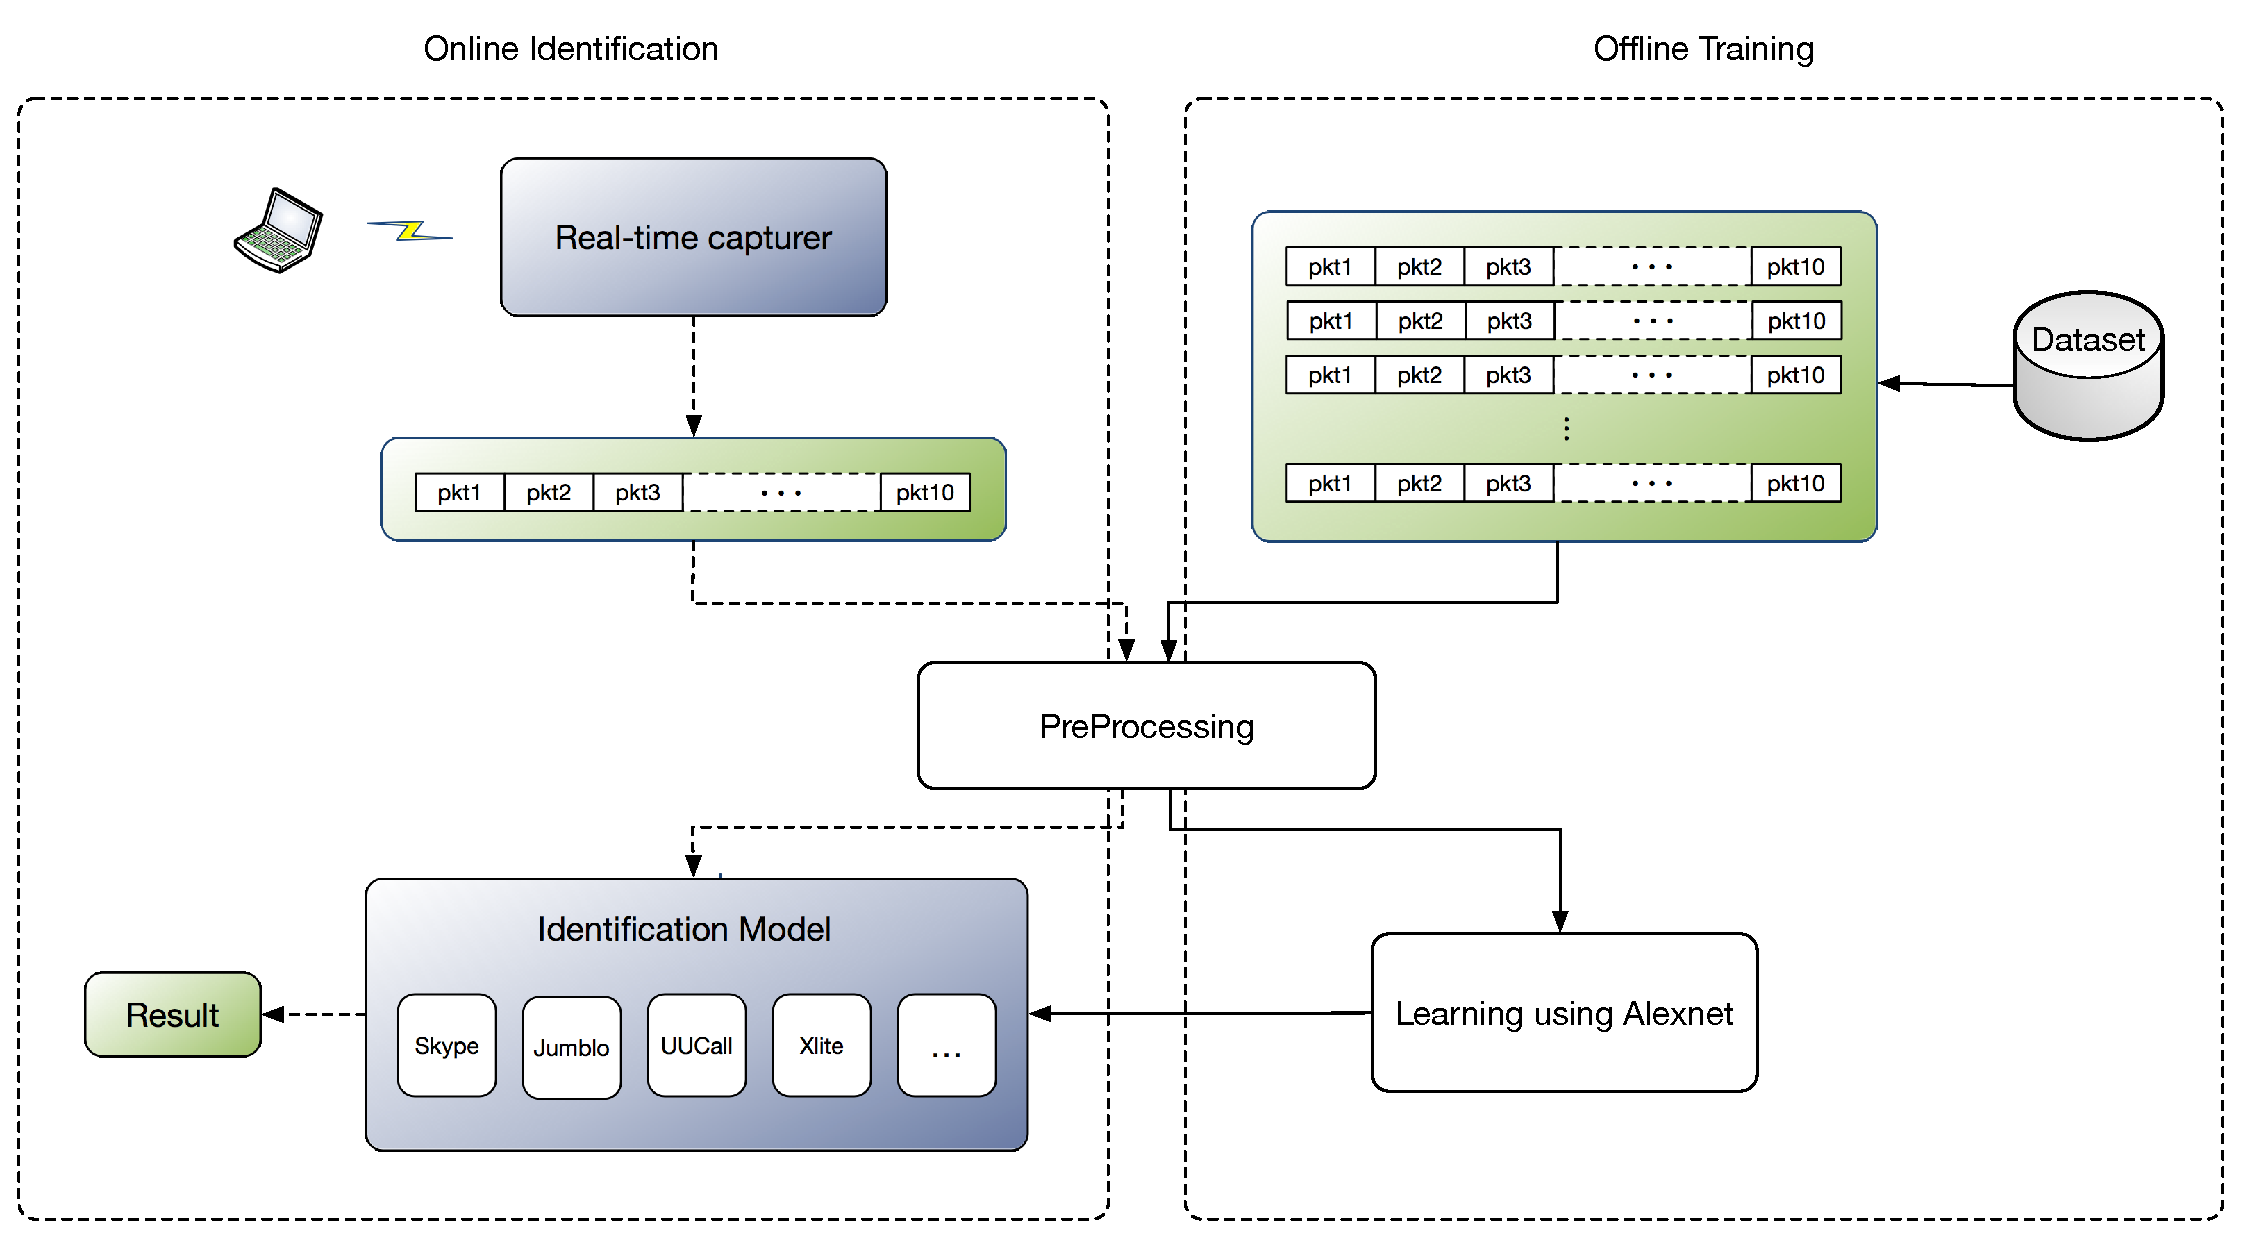
\includegraphics[width=0.47\textwidth]{architecture.eps}
\caption{Architecture of identification system.}\label{fig:architecture}
\end{center}
\end{figure}

\subsection{Offline Training}
In offline training phase, we extract features for 11 kinds of flows, which include 10 kinds of VoIP application flows and non-VoIP flows. Our goal is to maximize the accuracy of training and validation data. There are mainly 2 procedures, data preprocessing and model training. In preprocessing procedure, we random select k-packets with sliding window and label them with their application name. These k-packets and their labels will be processed into matrices as input of CLNN model. In training procedure, it is going to minimize the loss function to find an optimal function for identification. The output of training procedure is the feature set that we will use in real-time identification phase. We use the feature set to train VoIP application classifier, which is the final component of online identification phase.
%Offline training detailed in Figure~\ref{fig:offline_architecture.eps}.

%\begin{figure}[htp]
%\begin{center}
%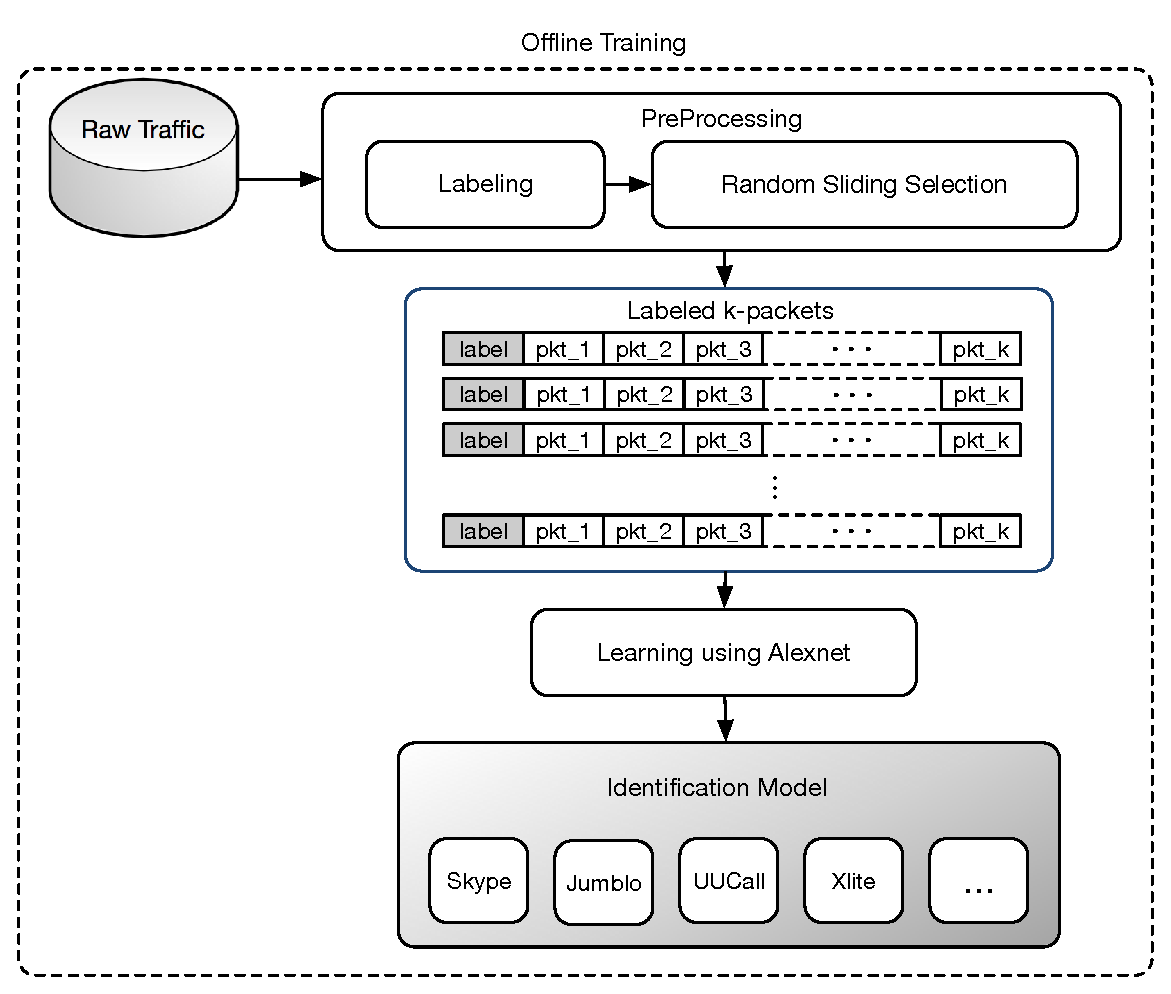
\includegraphics[width=0.45\textwidth]{offline_architecture.eps}
%\caption{Architecture of offline training.}\label{fig:offline_architecture.eps}
%\end{center}
%\end{figure}

\subsection{Online Identification}
Online identification is based on the output of offline training. In this phase, we build flows for traffic in large-scale network. We parse IP address and UDP port as its key for each packet. We maintain a key-value database for these keys. If the value of the corresponding key has been set, the value is the identification result of the packet. If the value is empty, we search the key in pending flows database and add this packet into corresponding pending flow. When a pending flow is ready to be identified, it will be identified by identification model and set the identification result in database.  %Figure~\ref{fig:online_architecture.eps},

As the Figure~\ref{fig:architecture} shows, the number of pending flow key\_3 reaches k, it is ready to be identified. We show 2 captured packets whose keys are key\_1 and key\_2, packet corresponding to key\_1 will be real-time identified by querying the database, packet corresponding to key\_2 will be appended into its pending flow.

%Identification phase is the final part of our system. In this phase, we use identification model to identify the k-packet captured in real-time. This phase includes 3 procedures, inspection of VoIP traffic, preprocessing and identification. In inspection procedure, we detect beginning of a VoIP connection. After this, we capture a k-packet and convert it to matrix in preprocessing procedure. Then we input the matrix into identification model, the identification model give us the result which is a specific VoIP application.
%\begin{figure}[htp]
%\begin{center}
%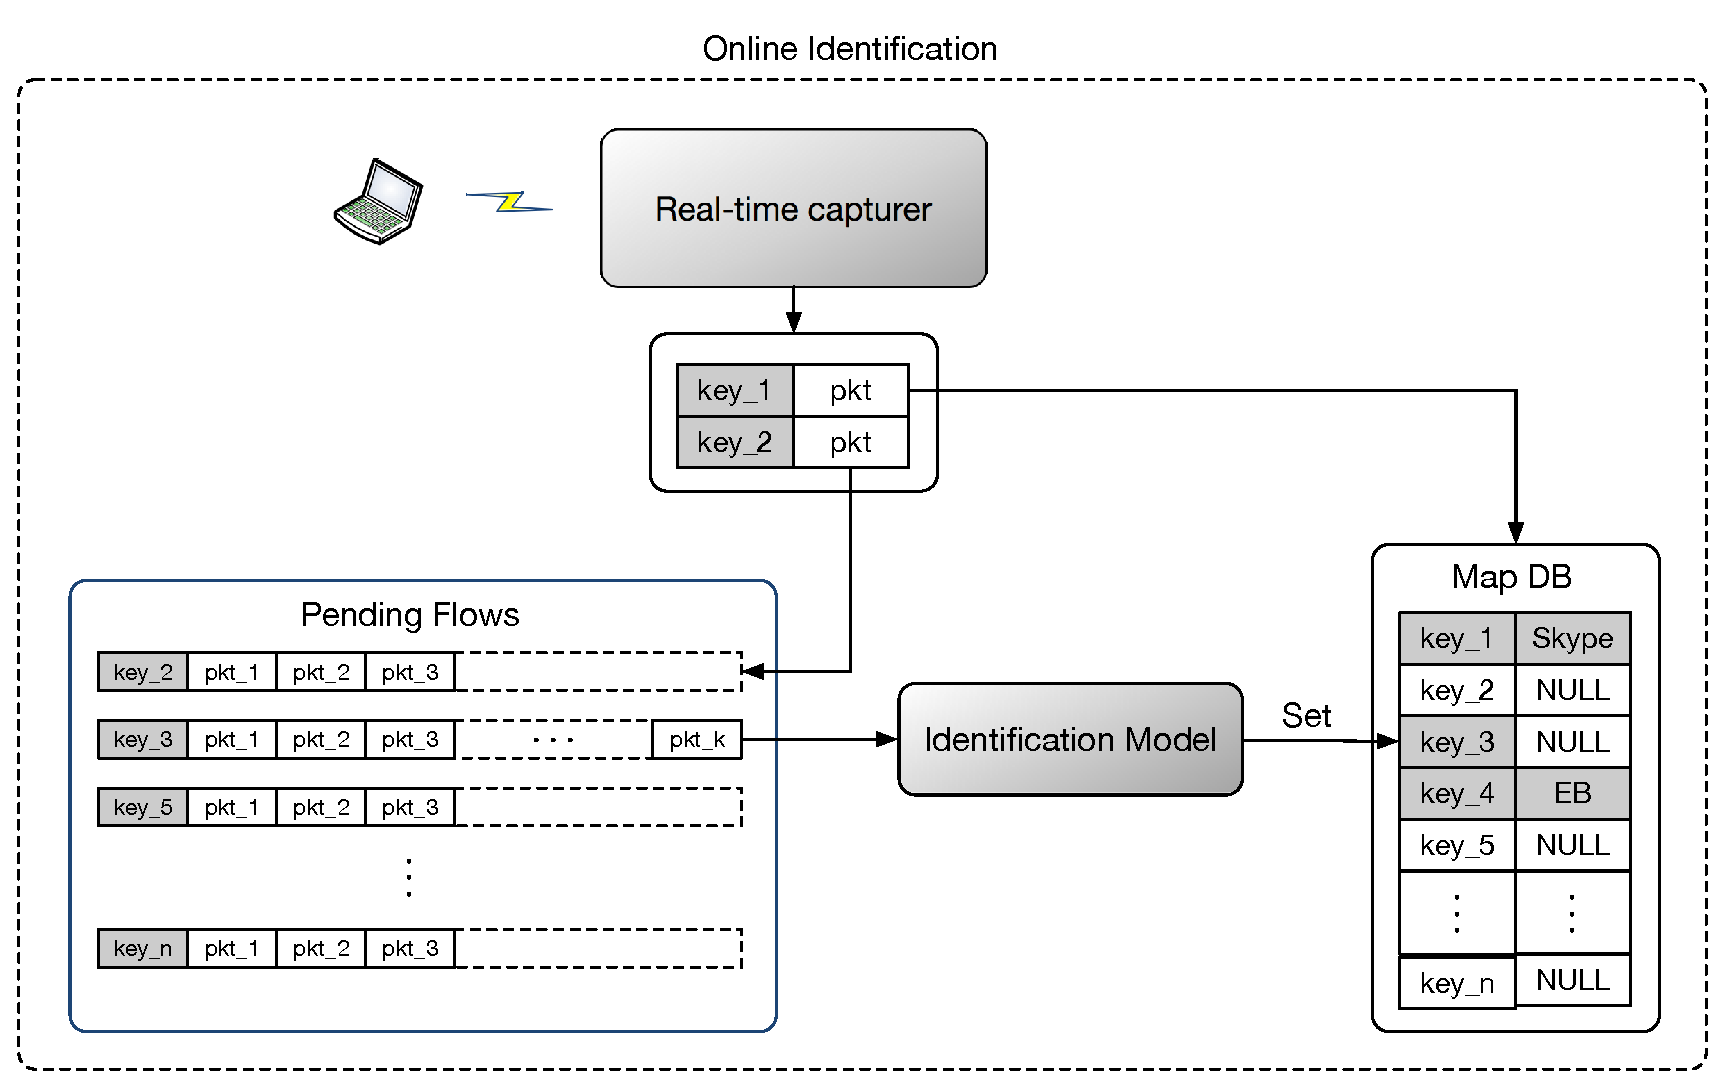
\includegraphics[width=0.45\textwidth]{online_architecture.eps}
%\caption{Architecture of online identification.}\label{fig:online_architecture.eps}
%\end{center}
%\end{figure}

\section{Traffic Collection and Processing}
\label{sec:trafficcollectionandprocessing}
Traffic collection is the beginning of all of the works. In order to get raw traffic of 10 VoIP applications mentioned above, we deploy 8 computers installed 10 kinds of VoIP applications. We installed 6 computers with Windows operating system, the others 2 computers installed with Linux operating system, because there are only 4 applications can be installed on Linux platform. We can establish ordinary VoIP calls among them, and all of them can dial the phone number directly. There are 4 cell phones ready to be called. We try our best to make calls from various places in the country to improve the credibility of our experiment.


%Traffic collection is the beginning of all of the works. In order to get traffic of 10 VoIP applications mentioned above, we deploy 8 computers installed 10 kinds of VoIP applications. We installed 6 computers with Windows operating system, the others 2 computers installed with Linux operating system, because there are only 4 applications can be installed on Linux platform. We can establish ordinary VoIP calls among them, and they can dial the phone number directly. There are 4 cell phones ready to be called.

For the purpose of labeling data easier, we use the process-based capture tool QPA under Windows operating system; We use tcpdump to capture traffic based on port, which can be known after process occupied. QPA provide GUI application under Windows OS, it is easy to use for capturing traffic for a single process. Under Linux platform, we need to analyze the ports VoIP
application uses, then we use command like "tcpdump -i eth\_name trans\_protocol port port_id" to capture traffic of specific ports. Because of process-based and port-based capture, it is easy to label raw traffic with their process name. Traffic from various video and game software will be labeled as non-VoIP traffic.

We need to construct our training dataset with captured raw traffic. We process the raw traffic to k-packets, we use sliding window to select k-packet into our dataset. The length of the window is k, and the next step is random. It ensures that our dataset isn't overly similar or vague. Figure~\ref{fig:dataset} shows how we select 4 k-packets for $k=10$. In this paper, a variety of CLNN models are trained according to different k, including 2, 4, 6, 8, 10, 20, 40 and 100. We have 4 steps to convert a k-packet to matrix. 1) Remove IP and UDP header; 2) Add 2 timestamps to each packet, one is the time difference from the first packet, the other one is the time difference from the previous packet; 3) Convert the k-packet to matrix on the basis of ASCII code; 4) Normalize the matrix. The length of VoIP packets is generally small around 50$\sim$210, so we set column of the matrix to 256. The row of the matrix is k, indicating a k-packet includes k packets.

%Before training with deep learning model, we need to preprocess packets to k-packet. In this paper, a variety of identification models are trained according to different k, including 2, 4, 6, 8, 10, 20, 40 and 100. To get different datasets for each k value, we set the size of sliding window equals k, and select random step length value from 1-k. Figure~\ref{fig:dataset} shows how we building dataset for $k=10$. There are 3 steps that we convert a k-packet to matrix. 1) Remove IP and UDP header; 2) Convert the k-packet to matrix on the basis of ASCII code; 3) Normalize the matrix. The length of VoIP packets is generally small around 50\~210, so we set column of the matrix to 256. The row of the matrix is k, indicating a k-packet includes k packets.
\begin{figure}[htp]
\begin{center}
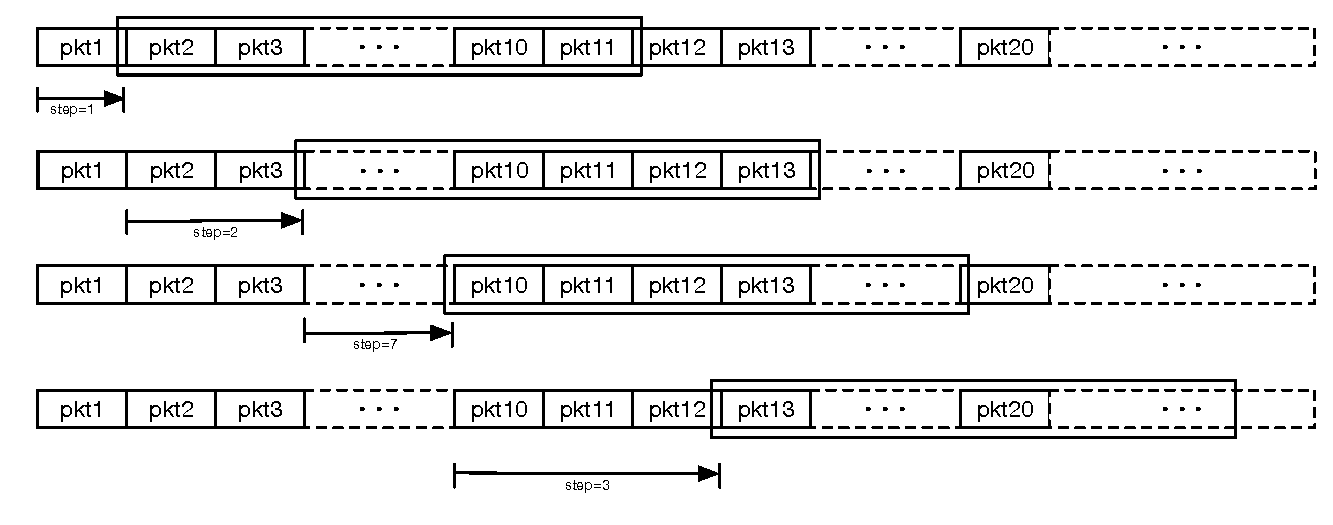
\includegraphics[width=0.45\textwidth]{dataset.eps}
\caption{How to process raw traffic to get k-packets(k=10).}\label{fig:dataset}
\end{center}
\end{figure}

\section{Learning with CLNN model}
\label{sec:learningusingdeeplearningmodel}
\subsection{CLNN model}
With the rise of artificial intelligence technology, more and more excellent deep learning models appear. The oldest is CNN (Convolutional Neural Network) proposed by~\cite{6}. The LeNet is a development of the CNN proposed by~\cite{7}.~\cite{8} published an incredible neural network called AlexNet, this model get the best performance in the ImageNet competition held in 2012.~\cite{9} proposed VGG. The GoogleNet make a daring attempt in the design of the network, which proposed by~\cite{10}.~\cite{11} proposed ResNet, which has a deeper network structure up to 152 layers.

%We compare CNN, AlexNet and GoogleNet with k set to 20 using a small part of dataset. The accuracy of CNN is above 94\%, the accuracies of AlexNet and GoogleNet are close to 1. GoogleNet costs more time and space than the other 2 models. We did comprehensive consideration about accuracy, efficiency, hardware requirements, data set size and other conditions, we decide to use AlexNet in the next further training. With the increase of dataset, we can use the models with a deeper network structure such as GoogleNet and ResNet.

We studied the above CNN models and were inspired by~\cite{clnn}, 
%we did comprehensive consideration about accuracy, efficiency, hardware requirements, data set size and other conditions, 
we employ a 8-layer CLNN model to train our data. Like many existing deep learning models, most of our ideas come from AlexNet. The difference is we embed LSTM for improving temporal features. Our model includes 8 layers, consists of 2 LSTM layers, 3 convolution layers and 3 fully connected layers. 
%We adopt ReLU (Rectified Linear Units) function as its activation function, and applies dropout in learning phase.

In our experiment, the inputs are matrices with size of k$\times$l, where k is number of packets used for k-packet, l is the column of matrix, we use 256. We adjust the filter kernel to 5$\times$5, and we change the padding type to same in each layer. The first 7 layers in the structure dropout the neural according to a probability of 0.5, the first 2 fully connected layers are activated using the ReLU activation function, and the last fully connected layer is activated using Softmax function. All LSTM layers use Tanh as their activation function when convolution layers use ReLU. We only keep max-pooling operation at 2\textsuperscript{nd} and 5\textsuperscript{th} layers, the pooling window set to 2$\times$2.

%The inputs are matrices with size of k$\times$l, where k is number of packets used for k-packet, l is the column of matrix, we use 256. In our experiment, several k values we select are not fit into AlexNet. So we do some adjustment on original AlexNet, we adjust the filter kernel to 5$\times$5, and we change the padding type to same in each layer. The first 7 layers in the structure dropout the neural according to a probability of 0.5, the first 2 fully connected layers are activated using the ReLU activation function, and the last fully connected layer is activated using Softmax function. We only keep a max-pooling operation in the last convolution layer, the pooling window set to 2$\times$2.

%\subsection{AlexNet}
%AlexNet includes 8 layers, consists of 5 convolution layers and 3 fully connected layers. AlexNet adopts ReLU (Rectified Linear Units) function as its activation function, and it applies dropout in learning phase. These 2 ideas shortens the training cycle so that it increases efficiency.

%The inputs of AlexNet are matrices with size of k$\times$l, where k is number of packets used for k-packet, l is the column of matrix, we use 256. In our experiment, several k values we select are not fit into AlexNet. So we do some adjustment on original AlexNet, we adjust the filter kernel to 5$\times$5, and we change the padding type to same in each layer. The first 7 layers in the structure dropout the neural according to a probability of 0.5, the first 2 fully connected layers are activated using the ReLU activation function, and the last fully connected layer is activated using Softmax function. We only keep a max-pooling operation in the last convolution layer, the pooling window set to 2$\times$2.
\subsection{Learning}
We use Softmax function as the activation function of the last layer. There are 11 types of traffic in our experiment, we calculate the posterior probability for unknown flow to identify its application type. Softmax function shows as
\begin{equation}
\hat P({V_i}) = softmax({V_i}) = \frac{{{e^{{V_i}}}}}{{\sum\limits_{j = 1}^n {{e^{{V_j}}}} }}
\end{equation}
where $({V_1},{V_2},{\rm{\cdot\cdot\cdot,}}{V_i},{\rm{\cdot\cdot\cdot}},{V_n})$ denotes the matrix to be inputted into Softmax in the 8th layer; $(\hat P({V_1}),\hat P({V_2}),{\rm{\cdot\cdot\cdot}},\hat P({V_i}),{\rm{\cdot\cdot\cdot}},\hat P({V_n}))$ is the output of the 8th layer, it is posterior probability distribution of k-packet, it is a vector with size of $1 \times n$; n is 11 in our experiment, it denotes the number of training traffic types.

During the training, we train data to find the most optimal weights to maximize the likelihood estimate of k-packet. To minimize the CCE (categorical cross-entropy), we have the formula as follow,
\begin{equation}
CCE({V_i}) =  - \sum\limits_{i = 1}^n {P({V_i}) \times \log (\hat P({V_i}))}
\end{equation}
where $P({V_i})$ denotes the real probability ${V_i}$, it is the target matrix generated according to the labels corresponding to the training data. $P({V_j})=1$, where j is the label corresponding to VoIP application that this k-packet belongs.$P({V_i})=0$,where $i \ne j$.

We use SGD (Stochastic Gradient Descent) optimizer to minimize the loss function in this paper, and apply nesterov momentum to update gradient after every iteration. The formula of gradient increment shown as follow,
\begin{equation}
\Delta {X_t} = \tau {M_{t - 1}} - \eta \nabla f({X_{t - 1}} + \tau {M_{t - 1}})
\end{equation}
where ${\tau}$ denotes the factor of momentum, ${\eta}$ denotes learning rate. ${g_t} = \nabla f({X_{t - 1}} + \tau {M_{t - 1}})$ is the gradient of transition point, where $\Delta {X_t}$ denotes the real decreasing displacement, ${X_t}$ denotes the position at time t, ${M_t}$ denotes the momentum at time t.

In our experiment, learning rate will decay after each epoch, decay rule shown as:
\begin{equation}
{\eta _i} = {\eta _{i - 1}} \times \frac{1}{{1 + \rho  \times i}}
\end{equation}
where ${\rho }$ denotes the decay factor, i denotes the number of epoch.

\subsection{Feature Set}
Our method is to get a more precise feature set for identifying VoIP traffic. The feature set extracted by deep learning is unreadable. The feature set is used to train classifiers with SVM, random forest, decision tree and naive bayes in our work, these classifiers are more real-time than the CLNN model. All of the classifiers trained with 4 machine learning methods achieved good accuracy. These classifiers will be used in real-time identification. 

\section{Real-time identification}
\label{sec:realtimeidentification}

In this section, we introduce how to real-time identify VoIP traffic with our identification system. There are 3 main components in real-time identification module. Capturer capture UDP packets and separate them into corresponding flows by IP address and UDP port. Filter follows several rules to filter out obvious non-VoIP flows. Classifier classifies flows into corresponding application type with extracted features.

%In order to capture the VoIP traffic in real time, we design a real-time traffic capturer. This capturer can capture UDP traffic and separate flows by IP address and UDP port. There is a rule-based filter to filter out non-VoIP flows preliminarily, the remaining flows will be sent to the classifier. The classifier will accurately classify flows according to application type.

%In most of VoIP applications, H.323 and SIP protocol are used for establishing and ending VoIP call. They both support call hold, call transfer, call forwarding, call waiting and some other supplementary services. So there are some researchers devote to monitor VoIP traffic based on call control signaling. It is no longer feasible to monitor VoIP traffic based on call control signaling. Here are several reasons: 1) SIP and H.323 protocols have their own development, and they support both UDP and TCP now. 2) The usage of ports is more and more irregular, it makes many identification methods useless. 3) More and more VoIP applications are encrypted to the traffic of call control. 4) For some VoIP applications, the server used for communication and that used for transmitting call control signaling are different. Due to these above reasons, it is hard to monitor VoIP call control signaling. These reasons also are our starting point to identify VoIP traffic with RTP/RTCP packets, all applications use RTP/RTCP protocol to transfer voice data.

The capturer maintain a pending flows queue and map packet into its matching pending flow using its IP address and UDP port. Figure~\ref{fig:flow} shows the details to separate flows by IP address and UDP port. If a packet cannot find the corresponding pending flow, it creates a new pending flow and adopt IP address and UDP port as its key. If a packet is appended into pending flow, and the number of packet reaches k, this k-packet will be sent to next component filter. The capturer guarantees that all captured packets are UDP packets, and the capturer can remove dead flows from pending flows queue. Flows whose number of packets doesn't reach k within limited time will be considered as dead flows.

\begin{figure}[htp]
\begin{center}
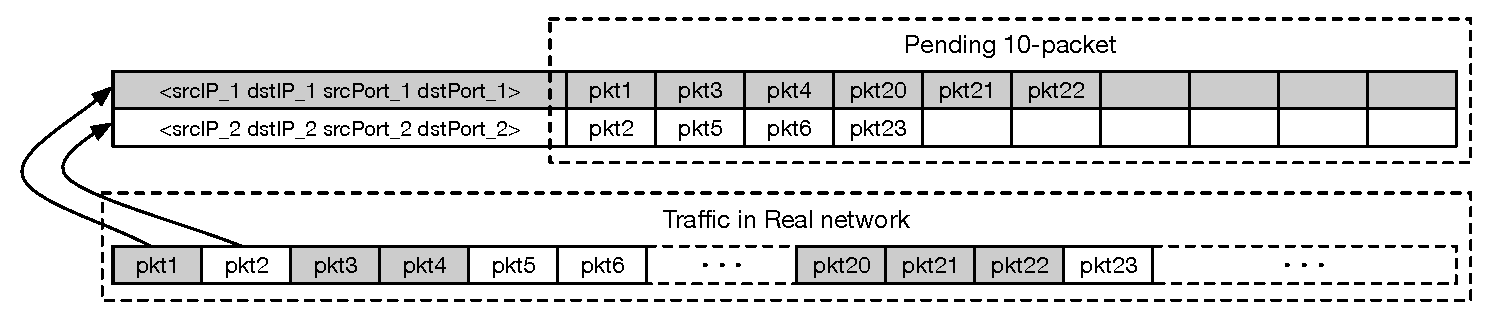
\includegraphics[width=0.45\textwidth]{flow.eps}
\caption{To separate flows by IP address and UDP port in real network.}\label{fig:flow}
\end{center}
\end{figure}

The second component is a rule-based filter, it receives k-packets sent by capturer. Because non-VoIP flows are no value to us, it will be filtered out to a certain extent. The remaining flows will be sent to next component to do further identification. We select benchmark values from our dataset and set several rules based on these benchmark values. Related algorithm and parameters are shown in Algorithm~\ref{algorithm:filter} and Table~\ref{tab:rules}.

\begin{table}[htbp]
  \caption{Benchmark value and threshold used in Algorithm~\ref{algorithm:filter}.}
  \label{tab:rules}
  \centering
  \begin{tabular}{l l l}
    \hline
    \textbf{} & \textbf{Symbol} & \textbf{Description}\\
    \hline
    1. & min\_mpl      &   Minimum of mean packet length in datatset\\
    2. & max\_mpl      &  Maximum of mean packet length in datatset\\
    3. & min\_pl      &   Minimum of packet length in datatset\\
    4. & max\_pl      &   Maximum of packet length in datatset\\
    5. & min\_miat      &   Minimum of mean inter-arrival time in datatset\\
    6. & max\_miat      &   Maximum of mean inter-arrival time in datatset\\
    7. & min\_iat      &   Minimum of inter-arrival time in datatset\\
    8. & max\_iat      &  Maximum of inter-arrival time in datatset\\
    9. & ${\lambda_1}$, ${\lambda_2}$      &  2 thresholds for upper and lower limits \\
    10. & ${\varrho}$    &   Proportional threshold for number of packets\\
    \hline
  \end{tabular}
\end{table}

\renewcommand{\algorithmicrequire}{\textbf{Input:}}
\renewcommand{\algorithmicensure}{\textbf{Output:}}

\begin{algorithm}[!h]
\caption{Algorithm to identify VoIP/non-VoIP Flows}
\label{algorithm:filter}
\begin{algorithmic}[1]
\REQUIRE Flow: k-packet
\ENSURE VoIP/non-VoIP
\IF{ ${\lambda_1}$min\_mpl $<$ mean packet length of current k-packet $<$ ${\lambda_2}$max\_mpl \textbf{and}  ${\lambda_1}$min\_miat $<$ mean inter-arrival time of current k-packet $<$ ${\lambda_2}$max\_miat  }
    \FOR {packet in k-packet}
       \IF{(packet length $<$ ${\lambda_1}$min\_pl )}
       	\STATE $ct\_pl\_l \gets ct\_pl\_l +1$
       \ENDIF
       \IF{(packet length $>$ ${\lambda_2}$max\_pl )}
       	\STATE $ct\_pl\_u \gets ct\_pl\_u+1$
       \ENDIF
       \IF{(packet inter-arrival time $<$ ${\lambda_1}$min\_iat )}
       	\STATE $ct\_iat\_l  \gets ct\_iat\_l+1$
       \ENDIF
       \IF{(packet inter-arrival time $>$ ${\lambda_2}$max\_iat )}
       	\STATE $ct\_iat\_u \gets ct\_iat\_u+1$
       \ENDIF
    \ENDFOR
    \IF{ct\_pl\_l $<$ ${\varrho}$k \textbf{and} ct\_pl\_u $<$ ${\varrho}$k \textbf{and} ct\_iat\_l $<$ ${\varrho}$k \textbf{and} ct\_iat\_u $<$ ${\varrho}$k}
        \RETURN $VoIP$
    \ELSE  \RETURN $non-VoIP$
   \ENDIF
\ELSE \RETURN $non-VoIP$
\ENDIF
\end{algorithmic}
\end{algorithm}

The k-packets that pass through filter successfully will be input into the third component classifier, the features used by the classifier are extracted in offline training phase. 4 kinds of classifiers are trained by SVM, Random Forest, Naive Bayes and Decision Tree, we select SVM classifier which have the best performance into our real-time system. The classifier takes k-dimensional matrix as input and output a vector whose size is $1 \times n$,  n denotes the number of VoIP applications that our identification model can identify. The vector indicates a k-packet's likelihood estimation for every VoIP application. The index of the maximum value in the vector is the identification result. The classifier can set the identification result in database, subsequent packets will be identified by querying the database. In the process of identification, one flow will pass through multiple k-classifiers when it grows up to different k stages, these classifiers will give their own identification results and corresponding possibilities. 

We adopt Apache Storm as our stream processing computation engine, and Apache Kafka as backup and load balance system to interact with networks. Figure~\ref{fig:storm} shows the Storm topology of our system. There is a Kafka Spout as the Kafka consumer client to consume the traffic from the network. A Bolt as capturer, a Bolt to distribute pending flows to next Bolt, the subsequent Bolt may be a filter or a classifier, which is determined by our settings based on k. The last Bolt RedisWriter is in charge of writing the identification results to the Redis database, and in order to get more accurate identification result, the result in database will be replaced by the classifier that gets higher probability.

\begin{figure}[htp]
\begin{center}
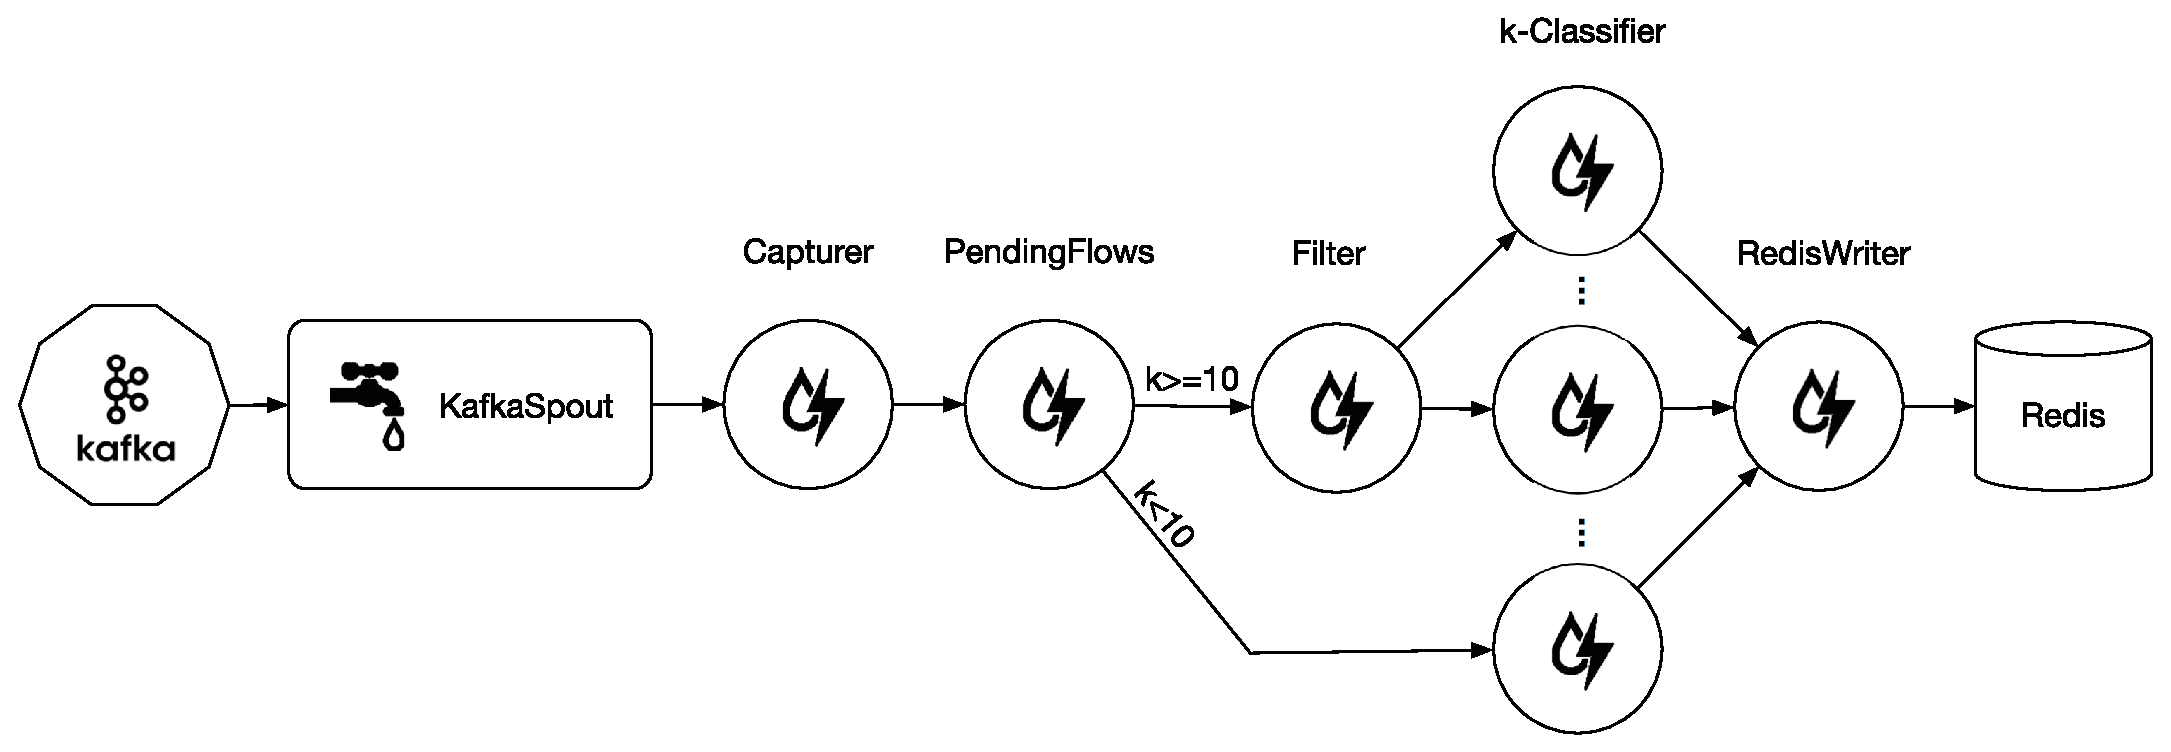
\includegraphics[width=0.48\textwidth]{storm.eps}
\caption{Storm topology of online identification system.}\label{fig:storm}
\end{center}
\end{figure}


%We input the matrix into identification model, it will output a vector whose size is $1 \times n$,  n denotes the number of VoIP applications that our identification model can identify. The vector indicates that this k-packet's likelihood estimation for every VoIP application. The index of the maximum value in the vector is the identification result. We will set the value in map database and remove this flow in pending flows. We do not have a way to identify unknown VoIP applications for now, but we want to improve our system. So we will research the packets whose maximum likelihood is less than 0.9.

%In order to detect VoIP voice traffic in real time, we have some rules. We only monitor the packets whose transport layer's protocol is UDP, and their packet length is less than 256. We parse the UDP packet that meets our requirements by RTP or RTCP protocol. If the UDP packet can be parsed correctly, we will process this packet with 2 operations, append it into corresponding pending flow or search identification result in map database. If it cannot be parsed, we ignored it. Moreover, we ignore packet that is alone, it makes no sense to monitor it. It is easy but it works better than the way based on call control signaling.




%In order to detect VoIP voice traffic in real time, we have some rules. We only monitor the packets whose transport layer's protocol is UDP, and their packet length is less than 256. We parse the UDP packet that meets our requirements by RTP or RTCP protocol. If the UDP packet can be parsed correctly, we will store its IP addresses and UDP ports, which used for the coming RTP/RTCP packets. If it cannot be parsed, we ignored it. Moreover, we ignore packet that is alone, it makes no sense to monitor it. It is easy but it works better than the way based on call control signaling. Figure~\ref{fig:flow} shows the details to separate flows by IP addresses and UDP ports.


%After we capture enough k packets for identifying. The next step is to process k-packet to matrix. The rules are same as above. We skip it here. We input the matrix into identification model, it will output a vector whose size is $1 \times n$,  n denotes the number of VoIP applications that our identification model can identify. The vector indicates that this k-packet's likelihood estimation for every VoIP application. The index of the maximum value in the vector is the identification result. We do not have a way to identify unknown VoIP applications, but we want to improve our system. So we will research the packets whose maximum likelihood is less than 0.9.

\section{Performance evaluation}
\label{sec:performanceevaluation}
In this section, we introduce the dataset used in our experiment firstly. Secondly, we give the specific parameters used in the CLNN model. Finally, we show the experimental results and give the evaluation of the system performance.
\subsection{Dataset}
\label{sec:dataset}
We divide captured traffic into 2 dataset. We use CLNN model to train dataset1, and we use dataset2 to examine extracted features. The details of dataset1 used for training shown in Table~\ref{tab:traffic}.

\begin{table}[htbp]
  \caption{The details of dataset1.}
  \label{tab:traffic}
  \centering
  \begin{tabular}{l l l l}
    \hline
    \textbf{VoIP} & \textbf{Platform} & \textbf{Size(MB)}& \textbf{Num.(k=10)}\\
    \hline
    Skype      & Windows, Linux  & 3908.8  &  669984  \\
    UUCall      & Windows  & 2709.4  &  691566  \\
    KCCall      & Windows  & 3128.8  &  808224  \\
    ALTCall      & Windows  & 2795.2  &  692002  \\
    Jumblo      & Windows, Linux  & 3704.6  &  871468  \\
    Zoiper      & Windows, Linux  & 4418.1  &  677114  \\
    Xlite      & Windows, Linux  & 5165.3  &  638288  \\
    Eyebeam      & Windows  & 4524.7  &  616773  \\
    ExpressTalk      & Windows  & 4633.1  &  602637  \\
    Bria      & Windows  & 4476.0  &  598724  \\
    non-VoIP      & Windows  & 11324.5  &  973522  \\
    \hline
  \end{tabular}
  %\caption{The details of dataset1.}
\end{table}

The forth column shows the num. of k-packet where k is 10, definitely, we also process the dataset according to k is 2, 4, 6, 8 and so on. It decides the first dimension of the matrix that will be input into CLNN model. 80\% of the k-packets are used for training when 20\% used for validating in training pahse.

\subsection{Parameter Setting}
\label{sec:params}

The optimization algorithm SGD used in training phase is a learning rate non-adaptive algorithm, the setting of learning rate has a direct impact on the experimental results. We learn from the general experience of deep learning, and we adjust it according to our experimental results. The initial learning rate is set to 0.01, it decays after 2 epochs following the rules mentioned in section 6.3.  Nesterov updates based on the gradient, we set momentum factor to 0.9. We train 20 epochs using the dataset for the above 8 models, we set batch size to 100. With these parameters, we get satisfactory results for every model. Table~\ref{tab:params} shows the number and storage size of weights identification model.
\begin{table}
  \caption{The details of CLNN parameters.}
  \label{tab:params}
  \centering
  \begin{tabular}{l l l l}
    \hline
    \textbf{Model} & \textbf{Input\_Shape} & \textbf{Num. of Parm}&\textbf{Size(MB)}\\
    \hline
    k=2      & ${2 \times 256 \times 1}$  & 17,818,697  &87  \\
    k=4      & ${4 \times 256 \times 1}$  & 17,820,823  &87  \\
    k=6      & ${6 \times 256 \times 1}$  & 34,600,197  &154  \\
    k=8      & ${8 \times 256 \times 1}$  & 34,602,387  &154 \\
    k=10     & ${10 \times 256 \times 1}$  & 51,381,825  &221.6  \\
    k=20     & ${20 \times 256 \times 1}$  & 84,947,847  &355.8 \\
    k=40     & ${40 \times 256 \times 1}$  & 168,859,507  &691.3  \\
    k=100    & ${100 \times 256 \times 1}$  & 420,613,687  &1619.3  \\
    \hline
  \end{tabular}
  %\caption{The details of Alexnet parameters.}
\end{table}

\subsection{Experiment Results}
\label{sec:experimentresults}
The dataset listed in Section~\ref{sec:dataset} is used to train. With the parameter setting in Section~\ref{sec:params}, we get 8 feature sets for different k. The training and validating accuracies are shown in Table~\ref{tab:acc4models}.
\begin{table}
  \caption{The training and validating accuracy of 8 CLNN models.}
  \label{tab:acc4models}
  \centering
  \begin{tabular}{l l l l}
    \hline
    \textbf{Model} & \textbf{Loss} & \textbf{Train Acc.}&\textbf{Validate Acc.}\\
    \hline
    k=2      & 0.015865  & 0.995560  &0.996130  \\
    k=4      & 0.007670  & 0.997700  &0.997860 \\
    k=6      & 0.004933  & 0.998520  &0.999340 \\
    k=8      & 0.004393  & 0.998690  &0.999130 \\
    k=10     & 0.001159  & 0.999650  &0.999650  \\
    k=20     & 0.000546  & 0.999880  &0.999880 \\
    k=40     & 0.002920  & 0.999120  &0.999460  \\
    k=100    & 0.006689  & 0.997620  &0.998730  \\
    \hline
  \end{tabular}
  %\caption{The training and validating accuracy of 8 identification models.}
\end{table}

For the above 8 CLNN models, we use TPR (True Positive Rate) and FPR (False Positive Rate) to evaluate them. TPR reflects the probability of positive samples are identified correctly, and FPR reflects the probability of negative samples are identified as positive samples incorrectly. 
%TPR can be computed by Equation 5.
%\begin{equation}
%TPR = \frac{{TP}}{{TP + FN}}
%\end{equation}
%And FPR can be computed by Equation 6.
%\begin{equation}
%FPR = \frac{{FP}}{{FP + TN}}
%\end{equation}

\begin{figure*}[htp]
\begin{center}
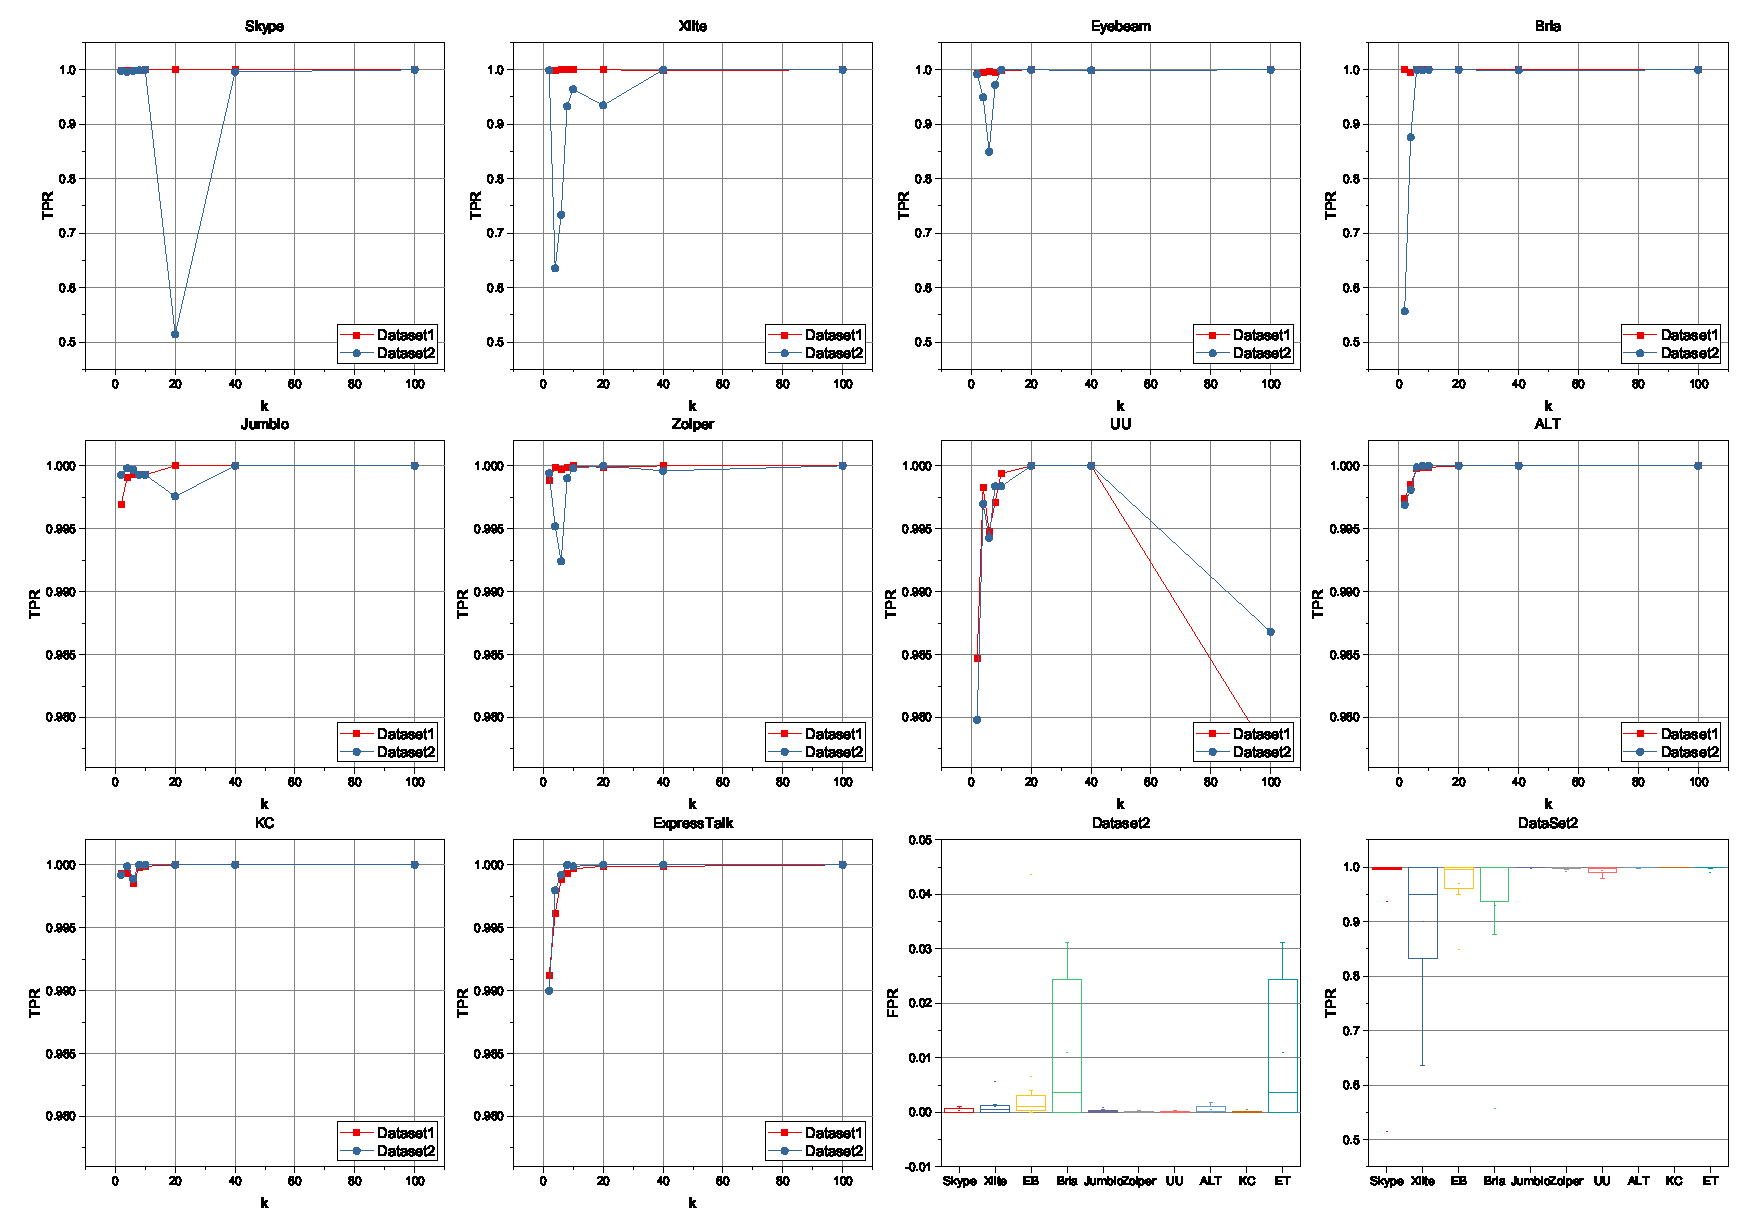
\includegraphics[width=1\textwidth]{fprtpr-hpcc.eps}
\caption{The performance of the 8 CLNN models shown by TPR and FPR.}\label{fig:fprtpr}
\end{center}
\end{figure*}

In our experiment, the identification rate for dataset1 is close to 1. When we examine these 8 models with dataset2, there are some outliers. They can be seen in the first 4 charts shown on Figure~\ref{fig:fprtpr}, model-20 for Skype, model-4 for Xlite and so on. This means these models that we trained is overfitting the dataset. In the future research, we consider add the L1-norm and L2-norm into our model, we will merge dataset2 into dataset1 to enlarge dataset to avoid overfitting. Apart from this, these charts show good performance to most of VoIP applications.

Figure~\ref{fig:tf} shows the probability distribution of true result and false result of dataset1 and dataset2, which true result means a k-packet is identified correctly and false result means a k-packet is identified incorrectly. It shows the maximum probabilities of true results are generally close to 1, and they are disperse from 0.2 to 0.98.
\begin{figure}[htp]
\begin{center}
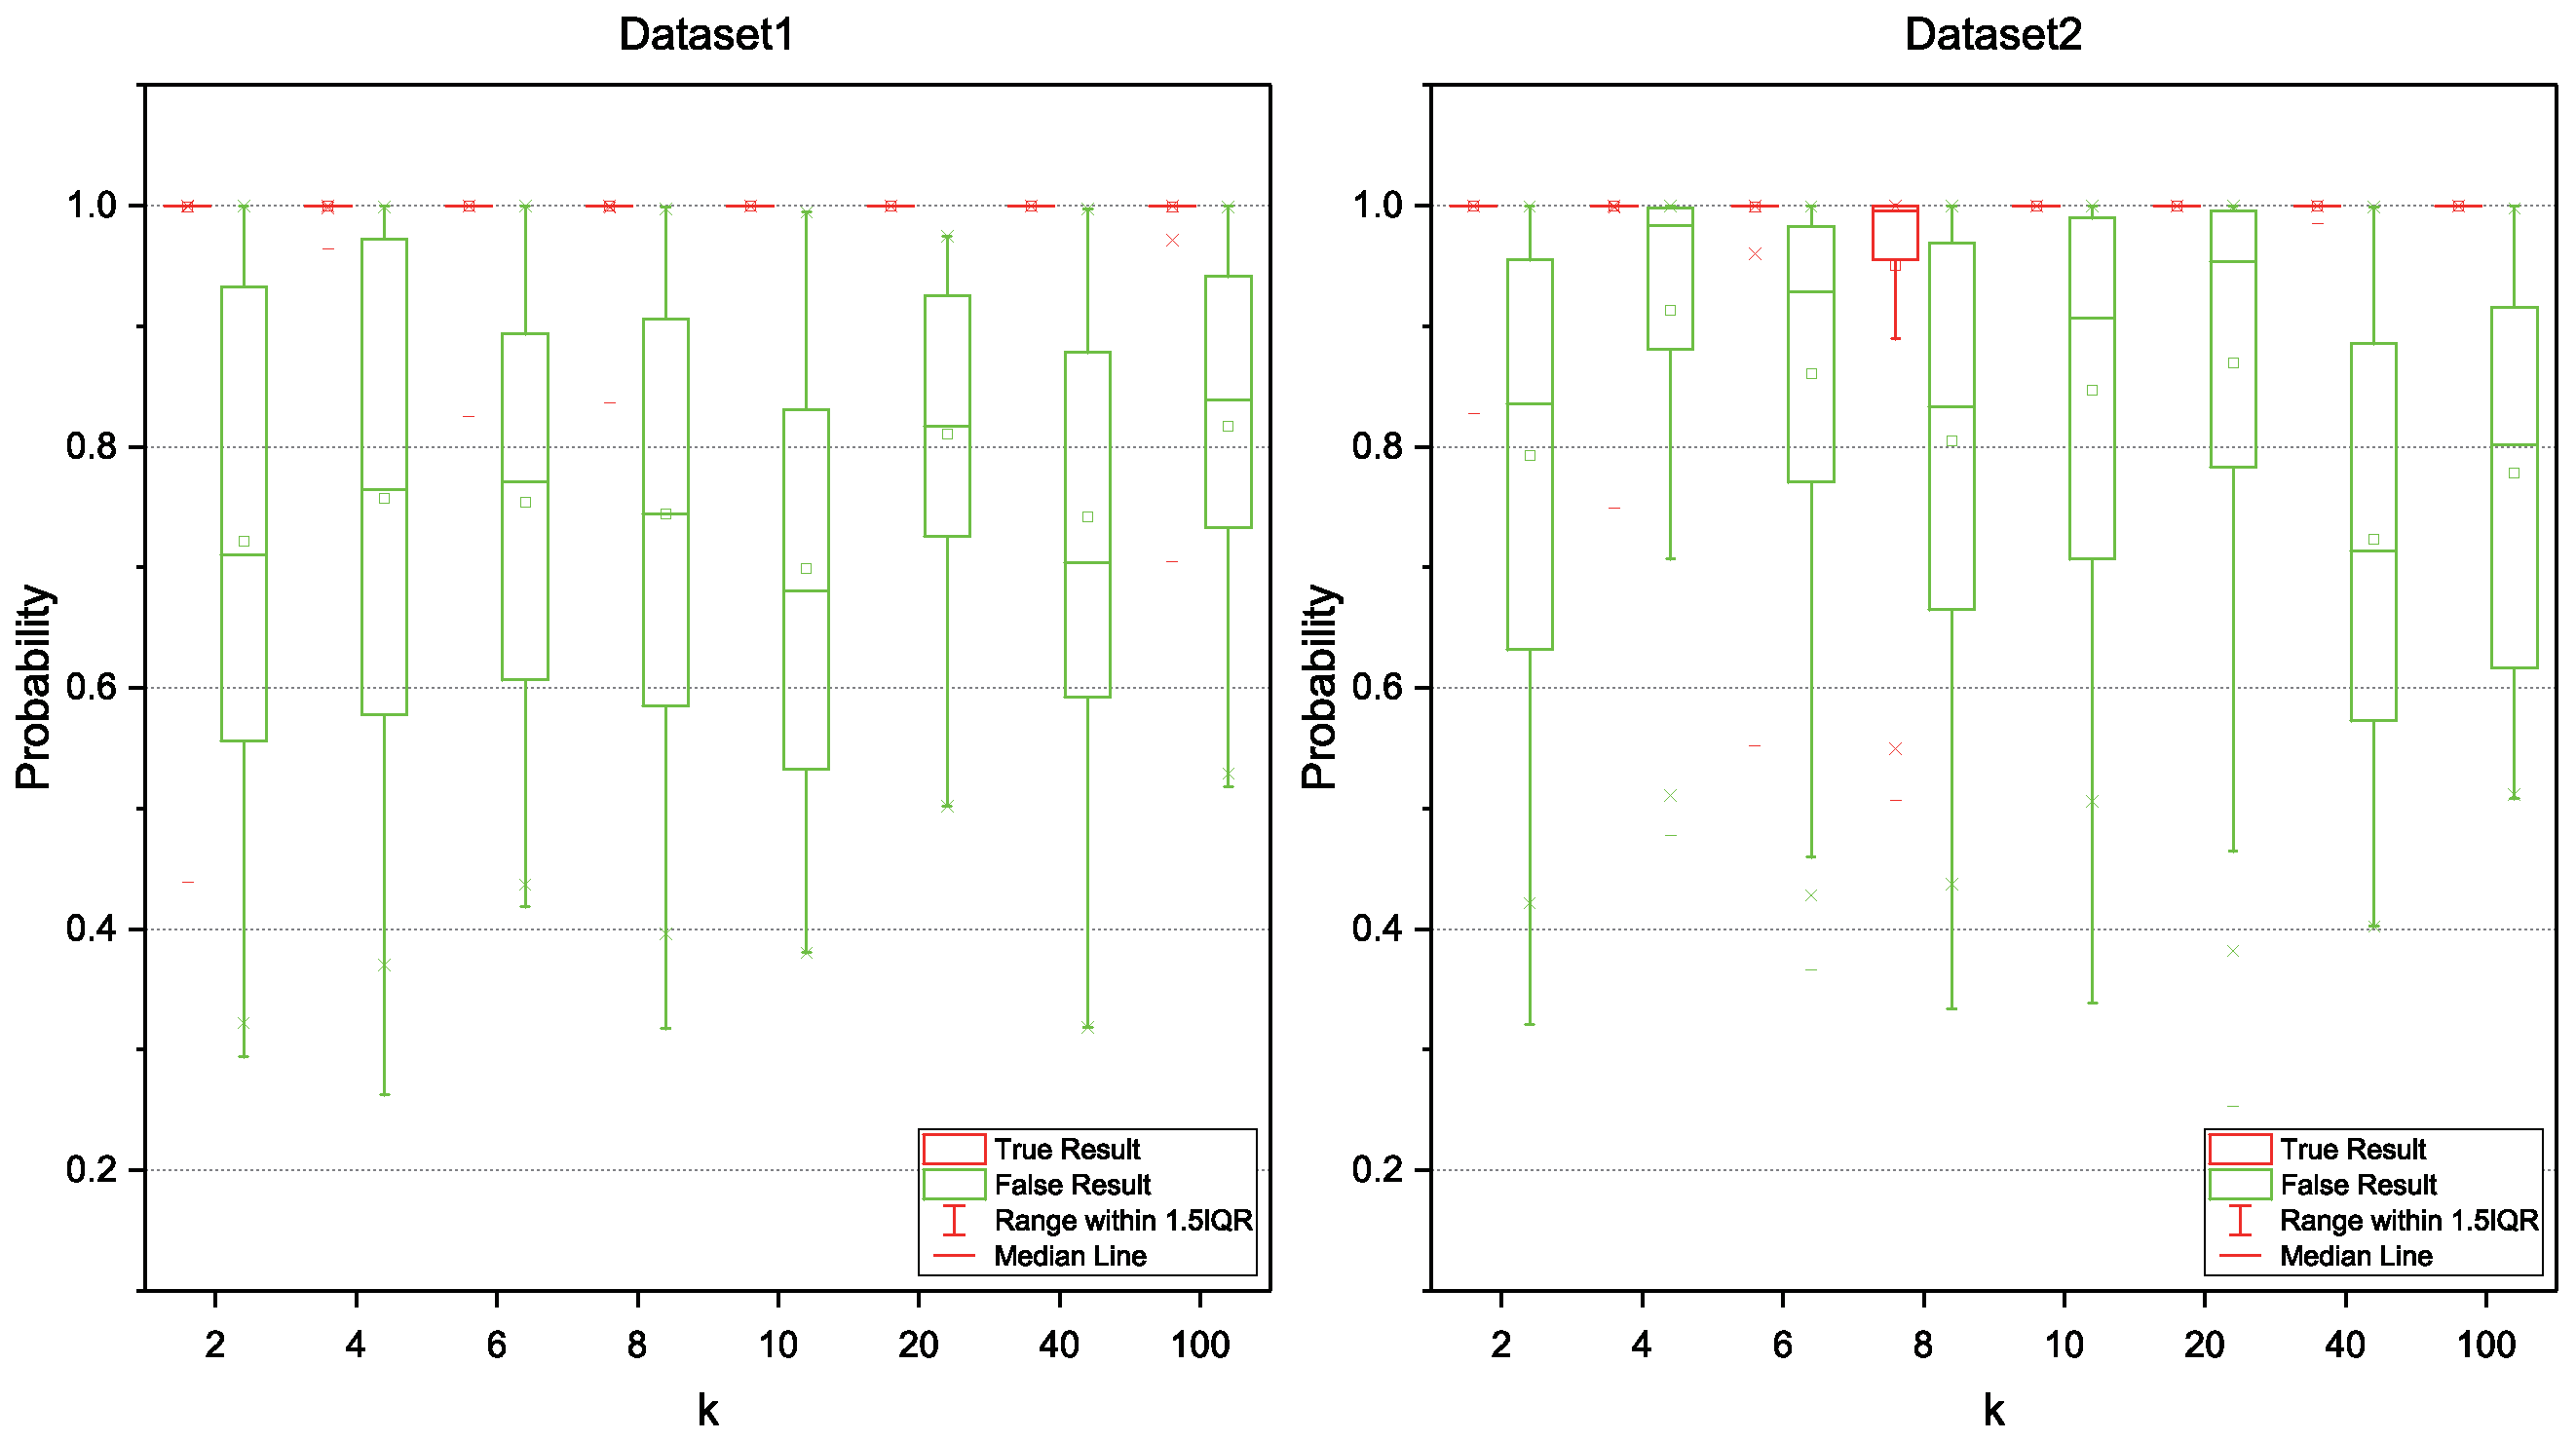
\includegraphics[width=0.45\textwidth]{tf.eps}
\caption{The probability distribution of true result and false result.}\label{fig:tf}
\end{center}
\end{figure}
We use the feature set we extracted by CLNN model to train classifiers with 4 machine learning models, the accuracy of them are shown in Figure~\ref{fig:ml}. The previous research we mentioned in Section~\ref{sec:relatedwork}, they use machine learning methods and feature set extracted by human to identify VoIP traffic. With our feature set extracted by deep learning, the accuracy is up to 98\% or even higher.
\begin{figure}
  \centering
  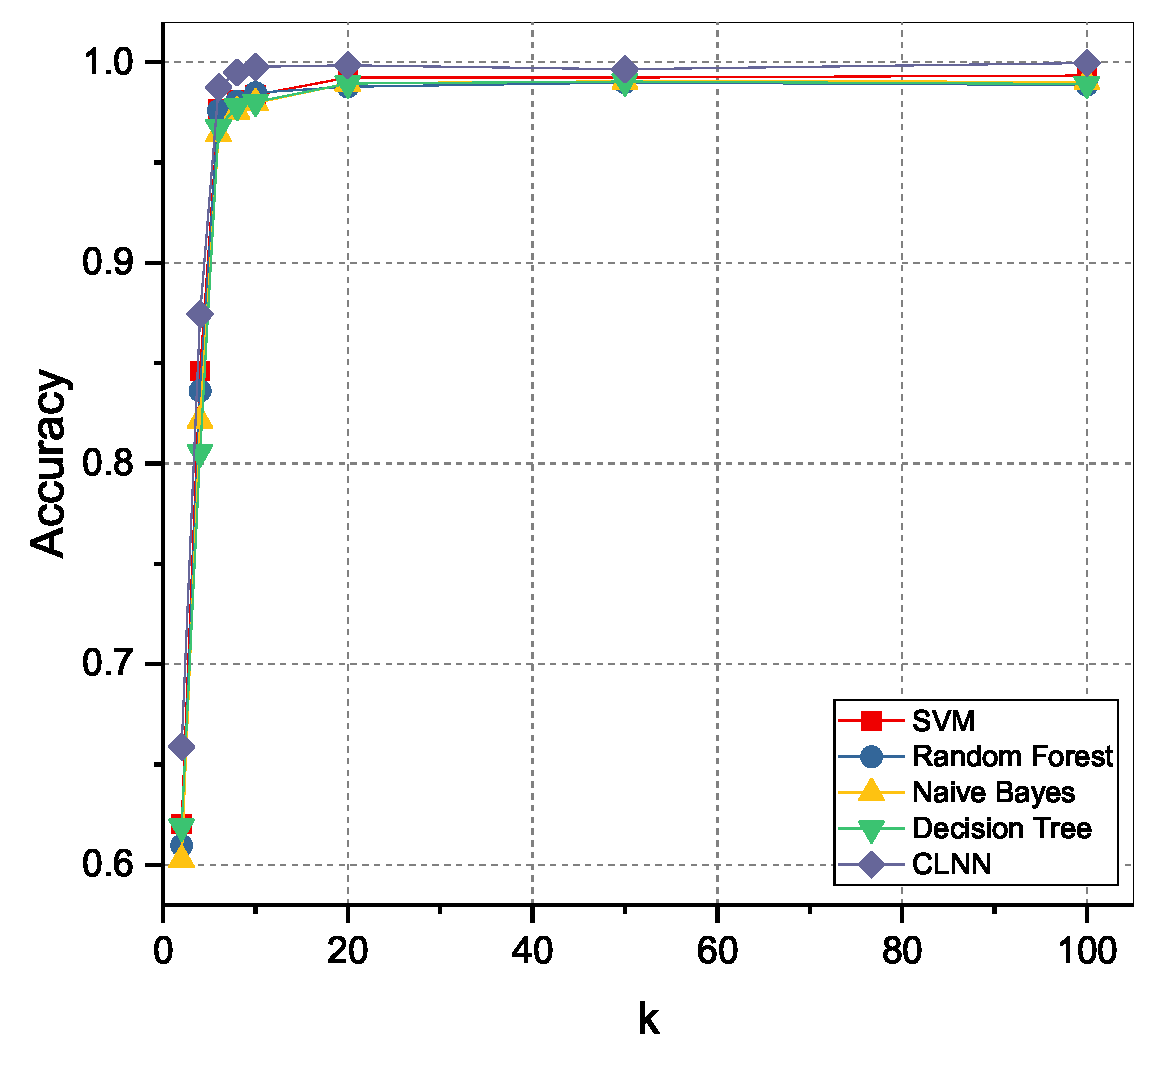
\includegraphics[width=0.45\textwidth]{ml.eps}
  \caption{The accuracy of 4 machine learning methods using extracted feature set.}
  \label{fig:ml}
\end{figure}

The identification efficiency of SVM is better than original CLNN model, we deploy classifiers trained by SVM into real network. We count the time consumed for identifying 100 flows with our system. Time consumed is shown on Table~\ref{tab:time4folws}. From this table we can see that it costs 3 seconds when k is 100, it is tolerate for a long call which lasts for minutes. For that call which end quickly, make identification time shorter is more valuable, classifiers with smaller k will obtain identification results faster.
\begin{table}
  \caption{The time consumed to identify 100 flows.}
  %\caption{The time consumed to identify 100 flows.}
  \label{tab:time4folws}
  \centering
  \begin{tabular}{p{0.7cm}p{0.5cm}p{0.5cm}p{0.5cm}p{0.5cm}p{0.5cm}p{0.5cm}p{0.6cm}p{0.6cm}}
    \hline
    \textbf{Model} & \textbf{k=2} &\textbf{k=4}&\textbf{k=6}&\textbf{k=8}&\textbf{k=10}&\textbf{k=20}&\textbf{k=40}&\textbf{k=100}\\
    \hline
    Time(s)      & 27.55  & 20.12  &29.09&30.53&48.00&73.62&141.33&309.51  \\
    \hline
  \end{tabular}
\end{table}

\section{Conclusion}
\label{sec:conclusion}
In our work, we propose a generic approach to real-time identify traffic of specific VoIP applications. We train classifiers with feature set extracted by deep learning and deploy these classifiers into our real-time identification system. The real-time system is deployed with stream processing computation framework Apache Storm and it shows good performance. For now, the VoIP applications mentioned in this paper only cover the applications that can directly dial cell phone, some other applications using the VoIP protocol may be judged as non-VoIP applications. Our next goal is to enrich the types of VoIP applications. Similarly, the types of non-VoIP traffic need to be as rich as possible too. Another weak point is that training is too time consuming, if network administrators want to add new VoIP applications, the feature set need to be trained again. Given that the main goal of our mission is to intercept specific VoIP traffic in real time, the current system has achieved new breakthroughs in identification accuracy.


\bibliographystyle{IEEEtran}
\bibliography{IEEEabrv,reference}


\end{document}
